
\section{Aufbau}

Das Kugelfall-Viskosimeter besteht aus einem Rohr, das die zu
untersuchende Flüssigkeit enthält, umgeben von einem Gefäß, durch das
mithilfe einer Umwälzpumpe Wasser gepumpt wird, um die Temperatur der
Flüssigkeit konstant zu halten. Dieses Gefäß wird von einem Stativ
gehalten, das die Apparatur drehbar lagert. Die Temperatur des
einströmenden Wassers kann über ein Thermostat eingestellt werden,

Zusätzlich befindet sich noch eine Libelle am Stativ, mit der
sichergestellt werden kann, das die Apparatur gerade steht.  Zur Messung
der Wasserbadtemperatur gibt es ein Thermometer am Kessel, der das
Wasser erhitzt.

Auf dem Rohr, in das die Kugel zur Messung eingelegt wird, befinden sich
drei Marken. Eine Skizze ist in Abbildung~\ref{fig:aufbau} zu sehen.

\begin{figure}
  \centering
  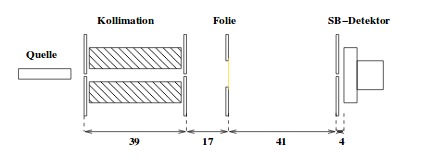
\includegraphics{aufbau}
  \caption{Schema der verwendeten Apparatur}
  \label{fig:aufbau}
\end{figure}
